\documentclass[10pt,a4paper]{article}

\usepackage{graphicx}
\usepackage[left=2cm,right=2cm,top=2cm,bottom=2cm]{geometry}
\usepackage[usenames,dvipsnames,svgnames,table]{xcolor}
\usepackage{placeins}

\newenvironment{ttSection}{\ttfamily}{\par}


\begin{document}

%\section{Annotations}

%\begin{itemize}
%\item \texttt{@NonParadigm(type)} : 'data' or 'active'

%\end{itemize}

\section{Analysis}

The current analysis phase takes an SCJ program, compiles it, and analyses it. The output of this section is a list of trees the represent the classes. Since this is SCJ agnostic, we intend to reuse this section. To check this, we have already compiled and analysed a Level~2 program using the current implementation of the tool. The list of trees is used during the translation phase, which we describe next.

\section{Translation}

The major difference between Level~1 and Level~2 programs is the ability to nest mission sequencers and so create a tiered program heirarchy, with clusters of missions and schedulables nested inside other missions. becasue of this key difference, we approach the translation in a heirarchical way. Figure~\ref{fig:translationFlow} shows a flowchart of the translation process. 

\begin{figure}[h!]
\begin{center}
\includegraphics[scale=0.5]{translation.pdf}
\caption{Flowchart of our Translation Process \label{fig:translationFlow} }
\end{center}
\end{figure}

At the top of the diagram we take in the SCJ Program and compile and analyse it, as we describe in the previous section. Then we begin the translation phase. Starting at the top of the program heirarchy, with the safelet, we find the tree belonging to each of the objects within the system. The safelet can be identified easily becasue there is only one in the program. The other objects are identified during the translation process, as we traverse the program's heirarchy, and are explored in that order to ensure that we caputre the heirarchy of the program correctly. beacsue eash class in the program is represented by a tree, we use the visitor pattern to traverse the different types of node that we might find in each tree and extract the information that we need for our translation, which we describe in Section~\ref{sec:translation}.

Upon discovery, each object (apart from the safelet) is assigned a unique identifier based upon the class's name. Multiple instances of a class result in multiple identifiers. This identifier is used in our model as a parameter to the processes representing that class. The location of the discovered objects within the program is important for the translation and is recorded.

\subsection{Find and Visit Safelet}

Becasue there is only one safelet in a program, to find the program's safelet we identify the class in the program that implements \texttt{javax.safetycritical.Safelet}.

\begin{ttSection}
Safelet = findSafelet()\\

findSafelet() = \\
for each class in the system, \\
if the class implements javax.safetycritical.Safelet then return it, else continue
\end{ttSection}

Once the safelet is identified we visit it and extract the contents of the \texttt{initializeApplication()} and \texttt{getSequencer()} methods, as well as any program-defined methods. 

The return values of the \texttt{getSequencer()} method are the top-level mission sequencers. The names of the classes that are top-level mission sequencers are collected and used in the next stage of the translation. 

Finally, the name of the safelet class is recorded for use in the translation of the high-level network of the processes in the model.

\subsection{Visit Sequencer}
\label{sec:sequencer}
This translation stage makes use of the top-level sequencer names recorded as the return values from the sfaelet's \texttt{getSequencer()} method. It is also used to translate any nested mission sequencers that are found during the visiting of schedulables. We discus this further in Section~\ref{sec:schedulables}.

We explore all of the missions that a mission sequencer can return and then all of the schedulables that each of its missions can register before moving on to the next mission sequencer. 

When visiting a mission sequencer we capture the contents of the \texttt{getNextMission()} method and any program-specific methods. Similarly to visiing the safelet, we collect the return values of the \texttt{getNextMission()} method for use in the next stage of the translation. 

Finally, we record the name of this sequencer and its location in the hierarchy. If it is rturned by the safelet's \texttt{getSequencer()} method, then is is a top-level sequencer. If it is returned by a mission, then it is a nested mission sequencer and its depth is recorded.

\subsection{Visit Mission}

This translation stage makes use of the collected names of the missions retunred by the \texttt{getNextMission()} method of a mission sequencer. Similar to visiting mission sequencers, we visit each mission returned by a particular mission sequencer and each of this mission's schedulables before moving on to the next mission. This is because we record each mission with its schedulables to form a cluster. 

When visiting a mission we capture the contents of the \texttt{initialize()} and \texttt{cleanUp()} methods, as well as any program-specific methods. 

To find the schedulables of a mission we find any class that may be registered during the mission's \texttt{initialize()} method. The names of these classes are collected and used in the next stage of the translation. 

We record the name of this mission, in preperation for pairing it with its schedulables as a cluster. We also record where in the hierarchy this mission resides. For example, if it is returned by a top-level mission sequencer, then it resides in Tier 0. 


\subsection{Visit Schedulable}
\label{sec:schedulables}

This stage of the translation takes a collection of names of the schedulables registered in a mission's \texttt{initialize()} method. We visit each schedulable in turn and check if it is a nested mission sequencer or some other kind of schedulable by checking if the schedulable extends \texttt{javax.safetycritical.MissionSequencer}. If the schedulable is a mission sequencer, then we use the same method described in Section~\ref{sec:sequencer}. Otherwise, we check if the schedulable is a managed thread or one of the three kinds of event handler.

When visiting a schedulable, which isn't a mission sequencer, we capture the \texttt{handleAsyncEvent()} method for event handlers or the \texttt{run()} method for managed threads, as well as any program-sepcific methods. 

When visiting a nested mission sequencer we vist the mission sequcner and then begin visitng its missions and their schedulables. A nested mission sequencer indicates a new tier in the program's hierarchy. 

Wehn we are visiting a mission's event handler or managed thread, we continue visiting schedulables from that mission until there are none left (or we find a mission sequencer) and then we move on to the next mission returned by the mission sequcner directly about this schedulable.

%what?
Once the mission sequencer in question has no more missions to explore, we return to the next mission sequencer about our current position. Once there are no more top-level mission sequcners we have explored all of the paradgim objects in the program and we can move on to the translation proper, described in the Section~\ref{sec:translation}.

\subsection{Non-Paradigm Objects}

Non-paradigm objects are objects in the program that do not extend classes or implement interfaces from the SCJ API. During the hierarchical exploration of the program, if any non-paradigm objects are instantiated then they are visited with a special visitor and their name is recorded separately.


\subsection{Components making Non-paradigm Method Calls}

A non-paradigm method call is when a method is called that is not specified in the infrastructure of SCJ, but is program-specific. Because we need to model them differently, we must identify when components make non-paradigm method calls. They can only occur during program-specific code, so we check each method called in application code to see if the class it is declared in is in the SCJ API or not. For methods that are in the SCJ API, they are paradigm method calls. Methods that are declared in the program are non-paradigm method calls. 

For example:
\begin{ttSection}
For each methodCall in applicationMethod, \\
if methodCall's declared class is not javax.safetycritical.Mission \\
then record it as non-paradigm\\
else\\
continue
\end{ttSection}


\subsection{Translate}
\label{sec:translation}

Translation occures in two stages, low-level and high-level. The low-level translation
translates the information gthered about each of the classes in the program during the prevous stages and produces the processes that represent them in our model. The high-level translation translates the information gathered about the program hierearchy and translates it into the clusters and tiers that make up the network of the processes that organises our model at the top-level.

Both stages of the translation are acheived using the Freemarker template enggine, whic takes a data model and a template and combines them to produce output. For the low-level translation, the information gatehrered from visiting each class in the program (as we described above) is used to produce a data model for that class. The relevent template is loaded and combined with the data model to produce our model. For the high-level translation, the information recored by each visitor about the position int he hierarchy of the class it is vising is used to construct a data model, the template is selected and combined with the data model to produce the high-level network that controls the processes in our model.


\end{document}